
%\begin{figure}[th!]
%    \centering
%    \includegraphics[width=1.0\linewidth]{figures/mlp.pdf}
%    \caption{The baseline architecture with MLP \protect\cite{harvard2019}.}
%    \label{fig:mlp}
%\end{figure}

\begin{figure*}[!th]
    \centering
    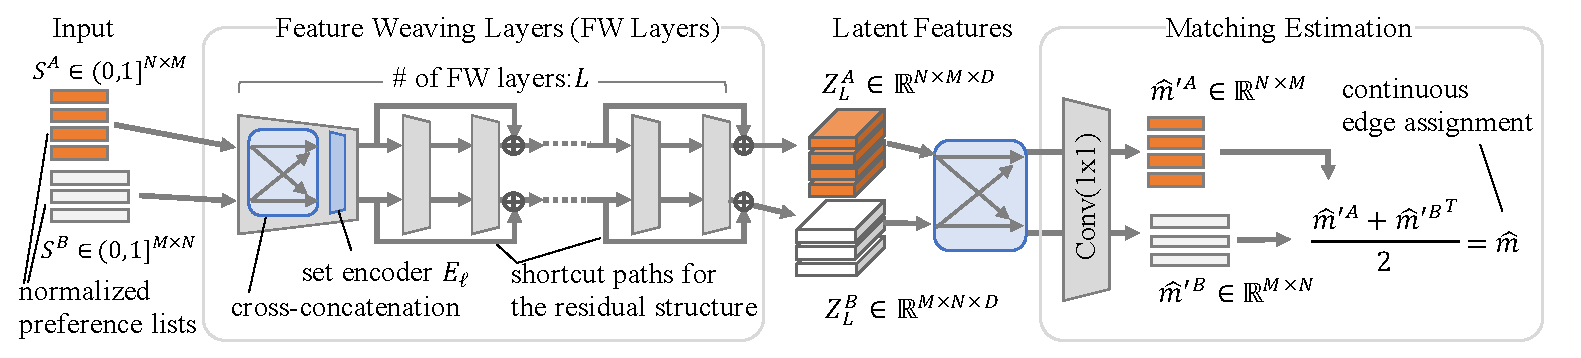
\includegraphics[width=1.0\linewidth]{figures/weavenet.pdf}
    \caption{WeaveNet architecture. $L$ feature weaving layers are stacked with shortcut paths to be a deep network. The encoded features are fed into Conv(1$\times$1) layer to obtain logits ($\hat{m}'^A$, $\hat{m}'^B$). The output $\hat{m}$ will be binarized in prediction phase to represent a matching.}
    \label{fig:weavenet}
\end{figure*}

\section{Deep-learning-based Fair Stable Matching}
%\ah{冒頭の文章，削りました}
\writtenby{Hashi}
%&In this section, we propose a novel neural network, {\it WeaveNet}, which encodes every edge of bipartite graph by common encoders while comparing features in $A\rightarrow B$ (weftwise) and $B\rightarrow A$ (warpwise) directions in a symmetric manner (\ref{ss:weavenet}).
%\jm{in Abst you used the word ``a shared set-encoder'', and here the word is ``a parameter-shared encoders''. I believe these words should be consistent (and more clear if possible)}
%We train the network with a continuous relaxation of the discrete objective functions and their conditions, which does not require any supervision by usually inaccessible ground truth (\ref{ss:relaxation}).

% 
\subsection{WeaveNet}\label{ss:weavenet}
\subsubsection{Input and Output Data Format}
We aim to realize a trainable function $F$ that outputs a matching $\hat{m}$, which is an $N\times M$ matrix.
As for the input, we firstly linearly re-scale\footnote{The details of this linear re-scaling are based on \cite{harvard2019} and described in \ref{ss:sf}. Note that sections numbered with capital letters appear in the supplementary material.} the rank of preference $p^*_{ij}~(*\in \{A, B\})$ ranged in $[1, N]$ into a normalized score $s^*_{ij}$ ranged in $(0, 1]$ to make it invariant to $N$, where 1 for the highest rank.
Then, we obtain the input as matrices $S^A$ and $S^B$, where $s^A_{ij}$ is the $ij$-element of $S^A$.


\subsubsection{Requirement, Intuition and Entire Model}
One of the required properties of $F:(S^A,~S^B)\rightarrow \hat{m}$ is to take all the agents' preference into account when determining the presence of each edge in the output $\hat{m}$. 
\cite{harvard2019} implemented this by multilayer perceptron (MLP), % (Fig.~\ref{fig:mlp}),
where
$S^A$ and $S^B$ are destructured and concatenated into a flat vector (with the length of $2N\hspace{-0.1em}M$) and fed to the MLP. Its output (a flat vector with the length of $N\hspace{-0.1em}M$) is restructured into a matrix $\hat{m}\in {\mathcal R}^{N\times M}$.
The MLP model, however, would face difficulties due to the following four problems.
\setlength{\leftmargini}{15pt}{
\begin{description}
	\setlength{\itemsep}{0pt}      %2. ブロック間の余白
	\setlength{\parskip}{0pt}      %4. 段落間余白．
	\setlength{\itemindent}{-15pt}   %5. 最初のインデント
	\setlength{\labelsep}{3pt}     %6. item と文字の間
 \item[(a)] Preference lists of multiple agents are encoded by independent parameters, though they share a format so that we could efficiently process them in the same manner.
 \item[(b)] MLP only supports a fixed-size input, so training different models for different cases of $N$ becomes mandatory.
 \item[(c)] $F$ should be permutation invariant, which means the matching result unchanged even if we shuffle the order of agents in $S^A$ and $S^B$, but MLP does not satisfy.
 \item[(d)] A shallow MLP model may be insufficient to approximate an exact solver for the NP-hard problem when $N$ is large.
\end{description}
}


To address the above weaknesses of MLP, we propose the feature weaving network ({\bf WeaveNet}) which has the properties of (a) {\bf shared encoder}, (b) {\bf variable-size input}, (c) {\bf permutation invariance}, and (d) {\bf residual structure}. The WeaveNet, as shown in Fig.~\ref{fig:weavenet}, consists of $L$ feature weaving (FW) layers. It has two streams of $A$ and $B$. In a symmetric manner, each stream models the agent's act of selecting the one on the opposite side while sharing weights to enhance the parameter efficiency. The shortcut paths at every two FW layers make them residual blocks, which allows the model to be as deep as possible. We explain its details as follows.

\begin{figure}[!ht]
    \centering
    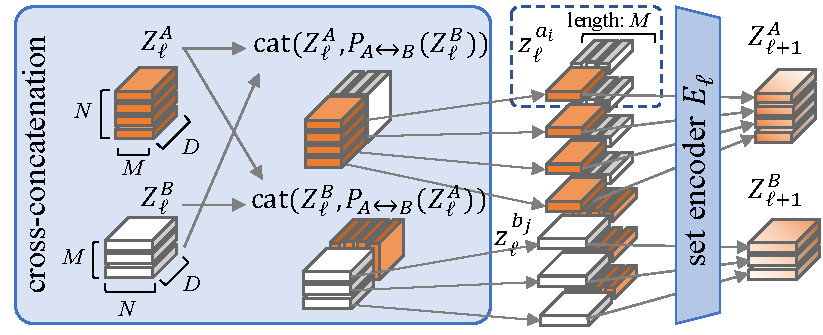
\includegraphics[width=1.0\linewidth]{figures/feature_weaving_layer.pdf}
    \caption{Feature weaving layer orthogonally concatenates the weftwise and warpwize components ($Z_\ell^A$ and $Z_\ell^B$) in a symmetric way (cross-concatenation). Then, the concatenated tensors are separated into $z_\ell^{\smash{a_i}}$ (or $z_\ell^{\smash{b_j}}$), which represents a set of outgoing edges from agent $a_i$ (or $b_j$), and independently fed to $E_\ell$.}
    \label{fig:feature_weaving_layer}
\end{figure}

\subsubsection{Feature Weaving Layer}
Fig.~\ref{fig:feature_weaving_layer} illustrates the detail of a single FW layer, which is the core architecture of the proposed network.
FW layer is a two-stream layer whose inputs consist of a {\it weftwise} component $Z^A_{\ell}$ and a {\it warpwise} component $Z^B_{\ell}$, where $Z^A_0=S^A$ and $Z^B_0=S^B$. 
The two components are symmetrically concatenated in each stream ({\bf cross-concatenation}). Then these concatenations are separated into agent-wise features, each of which is a set of outgoing-edge features of an agent (indicating the preference from that agent to every matching candidate).
These features are processed by the encoder $E_\ell$ {\bf shared by every agent in both $A$ and $B$}.
As for an encoder that can embed {\bf variable-size} input in a {\bf permutation invariant} manner,
we adopted the structure proposed in DeepSet \cite{deepset} and PointNet \cite{pointnet}, which consists of two convolutional layers with kernel size $1$ and a set-wise max-pooling layer, followed by batch-normalization and activation.
We refer to this structure as {\it set encoder}.
See \ref{ss:set_encoder} for visualization of the set encoder and its calculation cost.

\subsubsection{Difference from DBM}
Note that DBM \cite{gibbons2019deep} also satisfies the requirements (b), (c), and (d). The critical difference between WeaveNet and DBM is its parameter efficiency and the choice of the local structure $E_\ell$. DBM applies the weftwise and warpwise communications alternately in a single-stream architecture. Hence, each encoder is specialized in each direction. In our model, every encoder is trained for both directions, and thus it is twice parameter efficient.
See \ref{app:scope} to know how WeaveNet and DBM propagate the weftwise and warpwise communications.
Also, the local structure of DBM is sub-optimal to encode the relative identity of each outgoing edge among $N\times M$ pairs. 
We show the difference in performance brought by the local structure $E_\ell$ in the experiment section.

\checkedby{Jiaxin}{Hashi}
\subsubsection{Mathematical Formulations of WeaveNet}
The input $Z^A_\ell$ is a third-order tensor whose dimensions, in sequence, corresponding to the agent, candidate, and feature dimension, with a size of $(N, M, D)$.
Similarly, $Z^B_\ell$ has a size of $(M, N, D)$.
The {\bf cross-concatenation} is defined by function $P_{A\leftrightarrow B}$, which swaps the first and second dimensions of the tensor, and $cat(\{Z_1,Z_2,\ldots\})$, which concatenates the features of two tensors $Z_1,~Z_2$, as
\begin{equation}
\begin{split}
 Z'^A_\ell &= cat(Z^A_\ell,P_{A\leftrightarrow B}(Z^B_\ell)).
% Z^A_{\ell+1} &= (E_\ell(z^{a_i}_\ell)|0<i\leq N),
\end{split}
\end{equation}
$Z'^A_{\ell}$ is sliced into agent-wise features $z^{a_i}_\ell$ and we obtain $Z^A_{\ell+1} = (E_\ell(z^{a_i}_\ell)|0<i\leq N)$. We can calculate $Z^B_{\ell+1}$ in a symmetric manner (with the same encoder $E_\ell$).
%formulated by
%\begin{equation}
%\begin{split}
% z^{b_j}_\ell &= cat(Z^B_\ell,P_{A\leftrightarrow B}(Z^A_\ell))[j]\\
% Z^B_{\ell+1} &= (E_\ell(z^{b_j}_\ell)|0<j\leq M).
%\end{split}
%\end{equation}
%By stacking two or more FW layers, every element in the latent feature map can have a scope over the entire preference list (see Fig.~\ref{app:scope} for more detail). 

\checkedby{Jiaxin}{Hashi}
After the process of $L$ FW layers, $Z^A_L$ and $Z^B_L$ are further cross-concatenated and fed to the matching estimator (in Fig.~\ref{fig:weavenet}). It outputs a non-deterministic matching $\hat{m}$.
In the training phase, $\hat{m}$ is input to an objective function, and the loss is minimized.
In the prediction phase, the matching is obtained by binarizing $\hat{m}$.
In this sense, matching estimation through a neural network can be considered as an approximation by relaxing the binary matching space $\{0,1\}^{N\times M}$ (where 1 represents the edge selection while 0 for rejection) into a continuous matching space $[0,1]^{N\times M}$.

\subsubsection{Symmetric Property and Asymmetric Variant}
WeaveNet is designed to be fully symmetric for $S^A$ and $S^B$. Hence, it satisfies the equation $F(S^A, S^B)=F(S^B, S^A)^\top$.
This condition ensures that the model architecture cannot distinguish the two sides $A$ and $B$ innately. 
This property is beneficial when mathematically fair treatment between $A$ and $B$ is desirable. 
However, when inputs from $A$ and $B$ are differently biased (e.g., the two sides have different trends of preference), sharing encoders in two directions may degrade the performance.
To eliminate the bias difference without losing the parameter-efficiency, we further propose to \textbf{a)} apply batch normalization independently for each stream, and \textbf{b)} adding a side-identifiable code (e.g., 1 for $A$ and 0 for $B$) to $Z^A_0$ and $Z^B_0$ as a ($D$+1)-th element of the feature. We call this variant ``asymmetric''.


%%%%%%%%%%%%%%%%%%%%%%%%%%%%%
\subsection{Relaxed Continuous Optimization}\label{ss:relaxation}
Generally, a combinatorial optimization problem has discrete objective functions and conditions, which are not differentiable. To optimize the model in an end-to-end manner without inaccessible ground truth, we optimize the model by relaxing such discrete loss functions into continuous ones. 

Assume we target to obtain a fair stable matching that has the minimum $\SEq$, for example. Then, we have the following three loss functions.
\setlength{\leftmargini}{15pt}{
\begin{description}
	\setlength{\itemsep}{0pt}      %2. ブロック間の余白
	\setlength{\parskip}{0pt}      %4. 段落間余白．
	\setlength{\itemindent}{-15pt}   %5. 最初のインデント
	\setlength{\labelsep}{3pt}     %6. item と文字の間
 \item[$\loss_m$] conditions the binarization of $\hat{m}$ to represent a matching.
 \item[$\loss_s$] conditions the matching to be stable.
 \item[$\loss_f$] minimizing the fairness cost $\SEq$ of the matching
 %\ah{In the original optimization problem, this is the objective function while the above two were conditions. So better to avoid to say ``condition'' for this loss.}% conditions the matching to be fair by minimizing $\SEq$.
\end{description}
}
The overall loss function is defined as
\begin{align}
\hspace{-0.5em}    \loss_{\rm fsm}(\hat{m})&= \lambda_m\loss_m + \frac{1}{2}\hspace{-1.0em}\sum_{m\in \{\hat{m}^A,\hat{m}^B\}}\hspace{-1.3em}\bigl( \lambda_s\loss_s(m) + \lambda_f\loss_{f}(m)\bigr), \label{eq:lfsm}
\end{align}
where $\hat{m}^A = {\rm softmax}(\hat{m})$ and $\hat{m}^B = {\rm softmax}(\hat{m}^{\top})$. 

An advantage of learning-based approximation is its flexibility. We can modify the above loss functions to easily obtain other variants. For example, removing $\loss_{f}$ in Eq.\eqref{eq:lfsm} leads to standard stable matching, and replacing $\loss_{f}$ with $\loss_{b}$ (which minimizes $Bal$) leads to balanced fair-stable matching, as follows:
\begin{align}
\hspace{-0.5em}    \loss_{\rm sm}(\hat{m}) &= \lambda_m\loss_m \label{eq:lsm} + \frac{1}{2}\hspace{-1.0em}\sum_{m\in \{\hat{m}^A,\hat{m}^B\}}\hspace{-1.3em}\lambda_s\loss_s(m),\\
%
\hspace{-0.5em}    \loss_{\rm bsm}(\hat{m}) &=  \lambda_m\loss_m + \frac{1}{2}\hspace{-1.0em}\sum_{m\in \{\hat{m}^A,\hat{m}^B\}}\hspace{-1.3em}\bigl(\lambda_s\loss_s(m) + \lambda_b\loss_{b}(m)\bigr). \label{eq:lbsm}
\end{align}
%where $L_b$ is a loss function that minimizes $Bal$.

\subsubsection{Matrix Constraint Loss \texorpdfstring{$\loss_m$}{Lm}}
$\hat{m}$ can be safely converted into a binarized matching by column-wise or row-wise ${\rm argmax}$ operation when it is a symmetric doubly stochastic matrix \cite{harvard2019}.
To satisfy this condition, we defined $\loss_m$ with an average of the cosine distance as
\begin{equation}
\begin{split}
\hspace{-0.5em} {\rm C}(\hat{m}^A,\hat{m}^B)&=\frac{1}{N}\sum_{i=0}^N\frac{\hat{m}^A_{i*}\cdot\hat{m}^B_{*i}}{\|\hat{m}^A_{i*}\|_2\|\hat{m}^B_{*i}\|_2}\\
%
\hspace{-0.5em} \loss_m(\hat{m}^A,\hat{m}^B)&=1-\frac{({\rm C}(\hat{m}^A,\hat{m}^B)+{\rm C}(\hat{m}^B,\hat{m}^A))}{2},%\\
%&=1-\frac{N+M}{2NM}\sum_{\{i,j\}\in A\times B}
%\hat{m}'^A_{ij}(\hat{m}'^B)^{\top}_{ij}.
\end{split}
\label{eq:loss_c_p2}
\end{equation}
where $\hat{m}^A_{i*}$ means the $i$-th row of $\hat{m}^A$.
This formulation binds $\hat{m}$ to be a symmetric\footnote{Here the symmetry of $\hat{m}$ is defined by $\hat{m}_{i*} = \hat{m}_{*i}, i=1...M$ in case that $\hat{m}$ is not a square matrix ($N>M$).} doubly stochastic matrix when $\loss_m(\hat{m}^A,\hat{m}^B)=0$.
%This design of using cosine distance makes the loss exploration smooth on a hyper-sphere surface.
The advantage of this implementation against the original one in \cite{harvard2019} is described in \ref{ss:exp1_supp}.
%\jm{still not sure how to write the merit of this design.}\ah{I wrote some discussion to \ref{ss:exp1_supp}. How about just put the reference here?}
%while allowing rotate \mbox{$i$-th} column (and row) of $\hat{m}$ smoothly without increasing the loss. \jm{not sure what is ``rotate \mbox{$i$-th} column (and row) of $\hat{m}$''}
%Note that this implementation is different from the matrix constraint loss used in \cite{harvard2019} (see \ref{ss:lossc} in the supplementary material for details).

\subsubsection{Blocking Pair Suppression by \texorpdfstring{$\loss_s$}{Ls}}
As for $L_s$, we used the function proposed in \cite{harvard2019} as it is, which is 
\begin{equation}
\begin{split}
g(a_i;b_w,\hat{m}) &= \sum_{b_j\neq b_w}\hat{m}_{ij}\cdot \max(S^A_{iw}-S^A_{ij},0) \\ 
g(b_j;a_v,\hat{m}) &= \sum_{a_i\neq a_v}\hat{m}^{\top}_{ji}\cdot \max(S^B_{jv}-S^B_{ji},0) \\ 
\loss_s(\hat{m};I) &= \hspace{-1.0em}\sum_{(v,w)\in A \times B}\hspace{-1.0em}g(a_v;b_w,\hat{m})g(b_w;a_v,\hat{m}), 
\end{split}
\end{equation}
where $g(a_i;b_w,\hat{m})$ is a criterion known as ex-ante justified envy, which has a positive value when $a_i$ prefers $b_w$ more than any $b_j$ in $\{b_j|j\neq w,\hat{m}_{ij}>0\}$. This is the same for $g(b_j;a_v,\hat{m})$.
Hence, $\{a_v,b_w\}$ becomes a (soft) blocking pair when both $g(a_v;b_w,\hat{m})$ and $g(b_w;a_v,\hat{m})$ are positive. 

\subsubsection{\texorpdfstring{$\loss_{f}$ and $\loss_{b}$}{Lf and Lb} as Fairness Measurements}
$\loss_f$, $\loss_b$ minimize $\SEq(m;I)$, $Bal(m;I)$ in Table \ref{tab:costs}, respectively, and are defined as
\begin{align}
\loss_f(\hat{m};I) &= \frac{1}{N}|S(\hat{m};A) - S(\hat{m};B) |,\\
\loss_b(\hat{m};I) &= -\frac{1}{N}{\rm min} (S(\hat{m};A),S(\hat{m};B)),
\end{align}
%\jm{only $\loss_b$ has negative sign?}
where
\begin{equation}
~ S(\hat{m};A) = \sum_{i=1}^{N}\sum_{i=j}^{M} \hat{m}_{ij} \cdot {S^{A}_{ij}},~ S(\hat{m};B) = \sum_{j=1}^{M}\sum_{i=1}^{N} \hat{m}_{ij} \cdot {S^{B}_{ji}}.
\end{equation}
%\jm{Let's think about in which case we should use $m$ or $\hat{m}$.}
%which are an extension of $P(m;A)$ and $P(m;B)$ in Eq.~\eqref{eq:pref} for non-deterministic $m$ rescaled by $h$.


%In the prediction phase, we find the maximum likelihood matching in $\min(\hat{m}'^A,\hat{m}'^{B^{\top}})$ by the Hungarian algorithm.